\documentclass[conference]{IEEEtran}
\IEEEoverridecommandlockouts
% The preceding line is only needed to identify funding in the first footnote. If that is unneeded, please comment it out.
\usepackage{cite}
\usepackage{amsmath,amssymb,amsfonts}
\usepackage{algorithmic}
\usepackage{graphicx}
\usepackage{textcomp}
\usepackage{xcolor}
\def\BibTeX{{\rm B\kern-.05em{\sc i\kern-.025em b}\kern-.08em
    T\kern-.1667em\lower.7ex\hbox{E}\kern-.125emX}}
\begin{document}

\title{Individual Report: Long-term tracking of human skin areas on thermal images for monitoring vital signs\\}

\author{\IEEEauthorblockN{Seunghoi Kim}
\IEEEauthorblockA{\textit{MEng Computer Science} \\
\textit{University College London}\\
zcabski@ucl.ac.uk \\
}

}

\maketitle


\section{Introduction}
Object tracking has been researched for a long time and there are now a number of trackers that can accurately and robustly track objects. However, many studies are focusing on improving short-term tracking relative to long-term tracking which is different as long-term tracker must be able to handle well in conditions when the target goes outside of the frame for a long period of time, it detects the absence of target and re-detect the target when it re-appears \cite{b12}. Hence, long-term trackers consist of a short-term tracking component and a detector component for detecting target reappearance \cite{b12}. Since the tracking object may change its orientation, furthermore, the detector is required to update the tracking model appropriately.\\

Not only that, most of the state of the art trackers were studied under RGB domain, while not much of research was done on tracking thermal domain. However, thermal domain provides many advantageous data such as monitoring human vital signs unobtrusively and it is also invariant to the change in light illumination unlike RGB images, which means the tracking can be done even in a complete dark room. However, they tend to be blurrier on the edges and have lower resolution, which means the images are less textured and more difficult to find features for a robust tracking compared to RGB \cite{b3}. Although it is possible to apply many good existing RGB trackers on thermal images, Stojanovic et al. \cite{b10} states that they tend to perform worse than on RGB domain. For example, in VOT 2017 challenge, SRDCF came 3rd place in VOT-TIR challenge but came 40th in VOT challenge while MOSSEca came 34th in VOT challenge and 4th in VOT-TIR challenge\cite{b11}. This implies that there are needs of a new approach specialized for tracking under thermal images.\\

Hence, we introduce a novel method to improve the performance of tracking facial tissues under thermal domain by using synthetic images which are transformed from thermal domain to RGB domain using pix2pix designed by Isola et al. \cite{b1}. Since most existing trackers follow CNN structure, the attempts on image transition was done using CNN but the synthetic images were not accurate enough and blurry \cite{b1}. This is because CNN seeks to minimize the Euclidean distance between the ground truth pixels and the predicted, but the minimization is done by averaging all plausible outputs, which causes blurry effects. To overcome this, we used Conditional GAN by Zhang et al. \cite{b5}, which is a generative adversarial network where given a training set, it learns to generate synthetic RGB images as new data with the same statistics as the training set. Then, several state-of-the-art tracking algorithms developed for RGB images, such as TLD \cite{b9} and CSRT\cite{b11}, are applied onto the synthetic images to measure the performance of tracking. The results showed that in general, the performance of our proposed method was not significantly improved compared to tracking on raw thermal images. However, they appeared to perform much better when we tested on some particular regions, such as mouth and nostril.


\section{Personal Contribution}
\subsection{Data Collection}
Throughout the project, I have contributed in many areas.
My main project contribution was in the phase of preparing data sets for training GAN, which mainly deals with pre-processing data including gathering raw thermal images and performing image extraction, image quantization in order to be able to use for training. For training pix2pix model, we needed an enough collection of paired data of matching thermal and RGB images. This is because when another GAN model, cycleGAN by Zhu et al. \cite{b4}, trained on un-paired data was used, it generated less accurate results than the GAN trained with paired data. Initially, our team and I found the problem that there are not many thermal images for facial data available in open source. Hence, I decided to use a camera called ‘FLIR ONE pro’, to take facial images in RGB and thermal at the same time, which allows us to collect a paired data. This camera was only able to perform with Micro USB and with an app called ’FLIR One’, so instead, I used an OTG compatible USB gender to connect to my android phone, which uses USB-C. When I took images using ‘FLIR ONE pro’, I made sure that there was a good lighting condition, because RGB images are strongly affected by the surrounding illumination and good quality of original RGB images are required for generating good synthetic RGB images from raw thermal images during the cGAN training stage. Furthermore, I made sure that face was cooled enough to make clear distinctions between ambient temperature. The image taken using FLIR ONE is saved as JPG format, which contains both original RGB image and raw thermal sensor data embedded in the JPG metadata. I used a python library called ’FlirOneExtractor’ \cite{b16} to extract these metadata and separate the two images.

\subsection{Pre-processing}
After the extraction, to discard noises beyond 1.96 standard deviation in an image and separate the areas of background and the face more clearly, I applied an optimal quantization on the images using the TIPA library \cite{b7}, where the process is outlined in Cho et al. \cite{b6}. Once the quantization is applied on the image, the resulting image is converted into a grey-scale. As I mentioned in the earlier section, however, thermal images have disadvantages for use in face tracking as they have lower resolution compared to RGB images and blurrier on the edges \cite{b2}. Hence, there is a less texture and making it harder for good feature extractions. Therefore, I applied a sharpening filter, ’Laplacian Kernel filter’, to sharpen the image and make edges less blurry. This convolutional filter emphasizes the regions of large change in intensity by applying the second derivative filter after applying a Gaussian smoothing filter in order to reduce noises. Finally, since the original RGB image has a size of 1080*1440 and the thermal image has a size of 480*640, I resized the original RGB images to be the same as the thermal image. This is because pix2pix model takes a paired data of thermal and original RGB images of the same size as inputs. Although the reduction in the size of the image means the data in the image may be lost, which is not beneficial in tracking, we did not have any alternatives since the camera we used, ‘FLIR ONE pro’ provides 480*640 size of thermal images. Since our ROIs are small regions in a face, the data loss due to the reduction of the size of the image during preprocessing could be fatal to the performance. However, to resize the images, I did trial and error to find the closest size to the quantized thermal image and selected to use 0.55 ratio to resize RGB images. Hence, the resulting two images were able to be stitched together to put them in side by side as a single image file. To do this, I made python scripts and applied them over hundreds of images to be used for training data set. To increase the performance, I tried to gather as many different images possible including different orientations and different people. The more variety of data collected to train the model, the better the performance will be due to a greater number of different features. When the algorithms are applied, the output will look as figure 1 where the left image is the quantized thermal image and the right is the resized original RGB image.\\

\begin{figure}[htbp]
\centerline{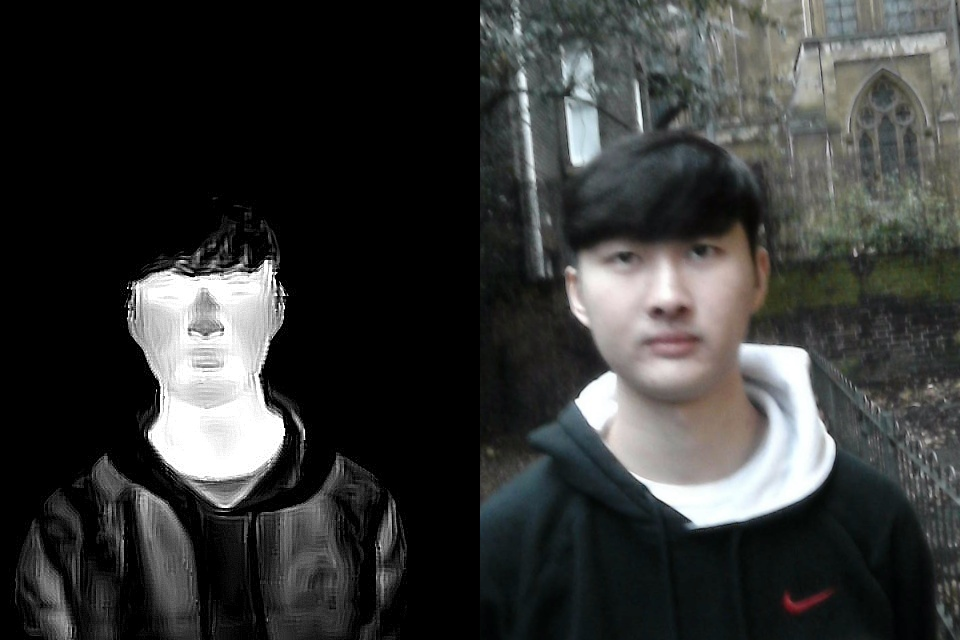
\includegraphics[scale=0.25]{92.jpg}}
\caption{Extracted images}
\label{fig}
\end{figure}

Furthermore, we applied normalization by dividing each image pixel value by 127.5 and then subtract 1 since the values for each pixel is in the range [0,255] originally. Hence, we get the new range of values for pixels as [-1, 1]. Finally, the dataset we collected is split in a most typical way, which is 75 percent training set and 25 percent validation set. Since the dataset we collected was limited and somewhat not adequate, the use of K-Folds cross validation might have been a better approach, since it results in a less biased model by assuring that every observation from the dataset has the chance of appearing in training and test sets.
\\
\subsection{Training GAN}
\begin{figure}[htbp]
\centerline{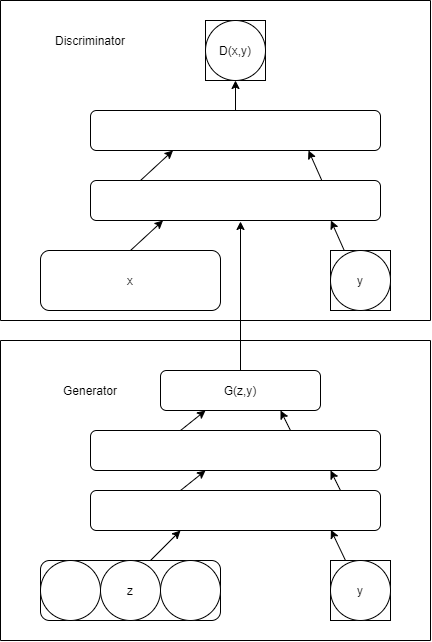
\includegraphics[scale=0.5]{cGAN architecture.png}}
\caption{Conditional GAN architecture}
\label{fig}
\end{figure}

Before implementing our model, it was crucial for me to understand the structure of GAN and how we can apply pix2pix and fit to our application. Our project focuses on using GAN which generates synthetic RGB images using ’Generator’ and then distinguish whether it is true or fake using ’Discriminator’. However, this is very difficult to get an accurate image close to the ground truth since if a single input image has a size of 512*512, then there are in total 512*512*3 possibilities if the output is in RGB. This is a reason why we needed to collect as much training data as possible. GAN trains by adversarial training which is composed with ’Generator’ and ’Discriminator’ that are used for producing a synthetic data and distinguish the true and false data respectively. Originally, we resized the input image to 256*256, but to increase the quality of our output, we increased the input size to 512*512 later on.\\
As shown in the figure 2, the Generator first generates a synthetic image using the random noise vector, z, along with the condition y. Then, the discriminator will decide whether this image is true (1) or fake (0) based on the real image x and Generator will be updated via Discriminator. When this whole forward and backward passes are completed, it is equivalent to one epoch and we used 100 epochs for training whereas Isola et al. \cite{b1} used 200 epochs. But we had to be careful in choosing the number of epochs as it could lead to overfitting, if the number of epochs is too high as we did not have enough training dataset. Hence, we sought to improve both Generator and Discriminator so that Generator generates a perfect synthetic RGB image and Discriminator has 0.5 probability of distinguishing whether the image is true or fake.\\

The reason behind using cGAN is that, Isola et al. \cite{b1} states that the resulting image using solely by L1 loss function tends to be blurrier than when both L1 and conditional GAN are used at the same time. Since, blurry images make harder for finding features for tracking, conditional GAN is more suitable for tracking purpose. Hence, the loss function of our model is defined as a summation of conditional GAN loss function and L1 loss function where L1 function is defined as expectation of Euclidean distance between the synthetic image and the original image for every pixel. To measure the performance of our GAN model, we plotted a graph measuring cGAN and L1 losses every time it trains and in this case we plotted a graph for every 20 epochs and lower the error indicates the model performs better. \\

During the implementation, we also intensively researched about the architecture of Generator and Discriminator of pix2pix model. Generator in our model follows the structure of U-Net which follows Encoder-decoder shape but with skip connection added. Hence, we performed downsampling until a bottleneck layer which means the size of images get shrink until the bottleneck. The images are downsampled using the strides equal to 2, so that the size of image is downsampled by half in every layer until it becomes 1*1*512. However, downsampling causes feature losses since the resolution is lower and this is fatal when we try to track small ROIs such as nostril, so we added more filters and, in this example, we used 4*4 spatial filters to preserve 512 different features of each image we put in as an input. Since we added many layers for improving the performance, it could have led to overfitting problem. Hence, during upsampling, we applied dropout by 0.5 leading to reduction in computational cost and less parameters to learn as it drops 50 percents of inputs. Discriminator is implemented as a PatchGAN and basically, as the patch goes around, it tells whether it is true or false. As Isola et al. \cite{b1} states, a PatchGAN with the size 70*70 is used as it produces a sharp and better quality of image compared to other sizes of receptive field.  \\

Once we constructed our pix2pix model and applied it onto training images, initially the outputs were not adequate, and the errors were high. For example, when we set up epochs to 100, the error rate for cGAN and L1 losses did not reduce anymore. The error rate was still high but the further increases in epochs did not significantly drop the error. The graph of the error rate when we initially trained the model is shown in the figure 3 below.\\
\begin{figure}[htbp]
\centerline{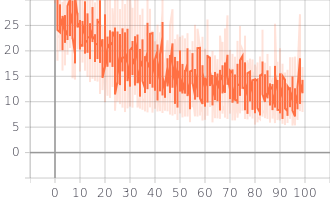
\includegraphics[scale=0.7]{gen_total_loss.png}}
\caption{Loss function throughout 100 epochs}
\label{fig}
\end{figure}
Looking at the graph, it implies that there is currently an underfitting as the training error is still high which means that it has high bias and low variance. Also, the rate of decrease in the error reduces as number of epochs increases, which tells us that we need to collect more training data to build more accurate model.\\
\subsection{Labeling}
Once we collected enough training dataset, I also took a part in labeling the ground-truth bounding boxes for various ROIs such as mouth in every testing image using an open source tool by Microsoft called Visual Object Tagging Tool (VOTT) \cite{b17}. We had in total five different sets which were (1) Slow Facial Movements (Nose), (2) Facial Movements with Partial Occlusion (Nose), (3) Rapid Facial Movements (Nose), (4) Minimal Facial Movements (Mouth), and (5) Minimal Facial movements (Nostril). The reason why we chose several ROIs is that some of regions in a face such as nose is already well distinguished from the other parts of a face in raw thermal images due to temperature difference, so we tried to choose different regions, in which it is not clear in thermal images, but can be well distinguished in synthetic RGB images. Finally we came up with mouth and nostril.

\begin{figure}[htbp]
\centerline{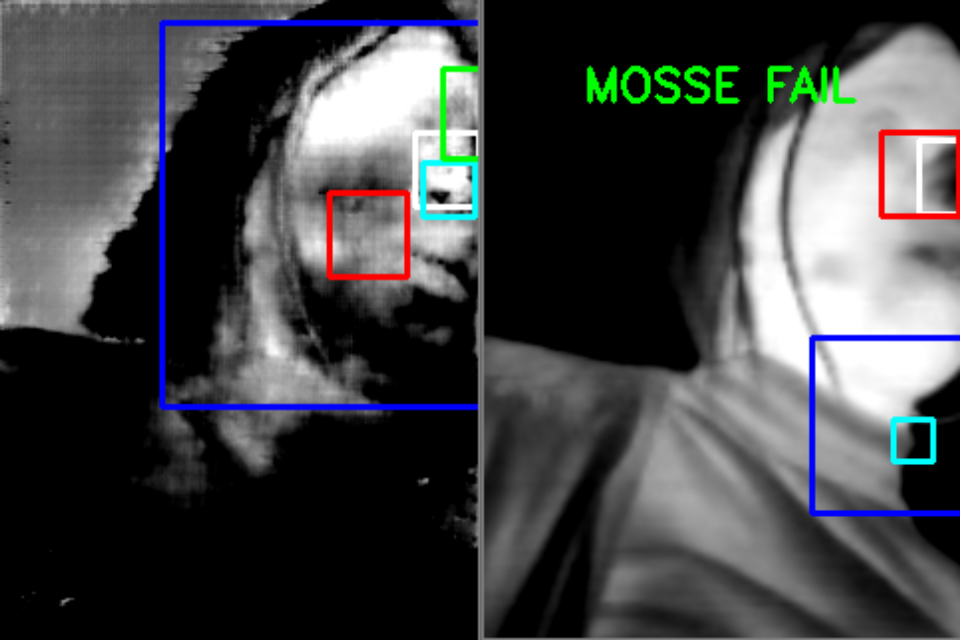
\includegraphics[scale = 0.25]{nostril.png}}
\caption{Tracking of nostril on synthetic RGB and thermal\cite{b20}}
\label{fig}
\end{figure}

To compare, we made sure that the synthetic images and raw thermal images were of same size since we saved the coordinates of the bounding box containing ROI in CSV file for every frame. Therefore, we resized all the images into 640*480 for RGB and thermal images. However, I confronted a problem during testing with the CSV file as the index or the frame number stored was not sorted properly. For example, they were laid out as 1.jpg, 2.jpg and then 10.jpg, 11.jpg...18.jpg, 19.jpg, 2.jpg, 20.jpg and so on due to the built-in sorting algorithms in VOTT. Hence, when we ran the benchmark, there were sudden changes in the motion of the ROI in between the frame 2 and frame 10 for example, which affected the performance of the trackers. Therefore, I had to re-sort these images manually, so that the images are shown in ascending orders properly. \\
Furthermore, to make the setting to be more suitable to our applications, we modified the function
\verb|’thermal_tracker()’| in TIPA library \cite{b7}. Originally, the user was able to select an ROI with a mouse and then tracks the ROI, but our modified version takes in an extra parameter, which is an array of the ground truth bounding boxes. Hence, rather than manually selecting the ROI in OpenCV, the ROI of the first frame of the video takes it as the initial ROI. This was done since we had to measure the accuracy metric by comparing the tracker’s output box with the ground truth bounding box throughout the video. \\


\subsection{Benchmark}
To benchmark the performance of state-of-the-art algorithms, we decided to use the algorithms that are available in OpenCV including some which performed well in VOT and VOT-TIR challenges. Hence, we were able to use these different algorithms to perform tracking at the same time. Then, by applying the algorithms we developed onto the sets of data given by Dr Youngjun Cho for test 1,2 and 3, we created multiple frames of synthetic RGB images for test dataset which add up to 600 frames. Finally, we established several metrics to compare the performance of trackers. Accuracy was calculated by Intersection over Union (IoU) which is the percentage of the bounding box that is overlapped with the ground truth, robustness was measured by counting how many times the tracker fails the target during tracking and finally expected average overlap (EAO). These three measures are the primary measures to analyze tracking performance in VOT challenges since 2015 \cite{b12}, so we concluded that this would be valid measures to compare the performance of our model as well.\\ For test 4 and 5, we only used 74 frames each, so this did not perfectly conform with our aim of project which is a long-term tracking. In vot 2017 challenge, it cites the definition of long-term sequence as, ”long-term sequence is a video that is at least 2 minutes long (at 2530 fps), but ideally 10 minutes or longer” by Mueller et al.\cite{b19}. This implies that the whole video must be at least in total 3000 frames for long-term tracking measurement. Although we did not perfectly meet the condition of the long-term tracking, there were needs to be a consideration of factors such as outbreak of COVID-19, lack of facial thermal dataset available we had and the fact that it was physically almost impossible to collect thousands of thermal and RGB images using ‘FLIR ONE pro’ camera in only few weeks.\\ During the testing stage, we initially included a performance on ‘Generated RGB with optimal quantization’ other than synthetic RGB and raw thermal images but decided to discard it since it did not contribute a significant improvement in tracking performance. Hence, as we proceeded the testing, we measured the performance of our independent variables which are the various tracking algorithms we used, Median Flow, TLD, MIL, MOSSE and CSRT on the raw thermal video and the synthetic RGB video. \\
By the suggestion of our supervisor, we have also tested, ’68 Landmark detection’ by Kazemi et al. \cite{b21} other than the object trackers. This tracker comprises with two steps which first uses a HOG with Linear SVM or Haar-cascade object detector to localize the face in an image and then applies a shape predictor for detecting the key facial parts on the face which then gives coordinates in x and y for the each key facial structure. There are in total 68 landmark points used to detect the face features. We have implemented this method using an open source library called ’dlib’ and applied it onto our testing images. Hence, we applied a pre-trained object detector for face detection. The output was considerably accurate even in some occlusions and the predictor was able to label the ROIs well.\\


\section{Results}
Before implementation, we expected the performance on synthetic RGB images would be better than thermal images. This was because most of the state-of-the-art tracking algorithms were developed under RGB images and they showed underperformance on thermal images. However, the results were different than what we initially expected due to the synthetic images having considerably large distortions and some blurring in the edges. As Moragn et al. \cite{b20} stated, the tracking in synthetic RGB generally was not significantly better than the thermal images. For test data 1, only CSRT and MIL trackers improved the performance in terms of accuracy. Note that, although the accuracy of MOSSE increased by 87 percents, we did not count this as an improved performance since the robustness was 0 which implies that it failed in every frames in the video. In test data 2, there was no improvement in any trackers while only slight improvements in performance for MIL and MOSSE for test data 3. Hence, for test data 4 and 5, we changed ROIs to nostril and mouth and the results turned out slightly better. We had a significant improvement in TLD which was almost double the performance under thermal and MIL for test data 4, while CSRT also improved in both accuracy and robustness in test data 5. Since out of these trackers we used, CSRT is the best performing tracker and has shown the most improvements in both metrics, the results can be considered to be significant. The more detailed results can be seen in Morgan et al. \cite{b20}.\\
Furthermore, we also tested Landmark detection using dataset 4 and 5. The results showed much more accurate face recognition on synthetic RGB images compared to thermal images. The tracker succeeded 41 images, failed in 33 images for RGB while it failed to track 73 images and succeeded in only one image for thermal images out of 74 images in total. The limitation of this tracker is that it showed a down-performance in handling a side view, but the tracker still detected accurately on the non-occluded regions which is much better than some object trackers which completely failed. The example of the tracking using ’Landmark detection’ \cite{b21} on RGB and thermal images are in the below. As you can see from the image, the detector is able to detect a face in RGB correctly, but completely fails and nothing is shown under the thermal image.

\begin{figure}[htbp]
\centerline{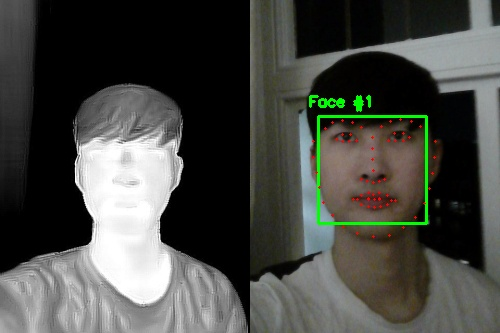
\includegraphics[scale = 0.45]{result.jpg}}
\caption{68 Landmark detection tested on thermal and RGB}
\label{fig}
\end{figure}


\subsection{Critical analysis of results}
There are multiple factors contributed to the results. However, the obvious reason is that the quality of raw thermal images we used were much better in the ROI we selected than the synthetic images. On the other hand, our synthetic RGB images were blurry by some extents which contributed as a major factor to the results. For example, for nasal region, we already had better distinctive features in the raw thermal images than the synthetic RGB images which influenced by lowering performance of RGB compared to the thermal images. Hence, we had to carefully select another ROIs again which we chose mouth and nostril. The results were much better than the previous attempts such as the accuracy of TLD was doubled up and the performance of MIL and CSRT also improved significantly.\\
Secondly, we had to resize the images by 512*512 during training GAN while the original RGB image taken had resolution of 1080*1440. If we used a higher resolution for training images, then we could have expected the performance of tracking to rise since there will be more features in a higher resolution. However, this has an opportunity cost as it will require much more time and power consumption. For real time applications, this is not satisfiable since there should not be any significant delay during tracking.\\
Furthermore, Isola et al., \cite{b1} states that they used 2975 images for training and trained for 200 epochs. However, for our project, we only used couple of hundreds of images for training. Hence, the output of the synthetic data was not as good as we expected. Also, during the implementation of our pix2pix model, we mostly followed the original structure. However, Ilyaivensky \cite{b13} states that Generator in GAN does not usually have dropouts. On the other hand, we had dropouts in upsampling in Generator which might have contributed in producing blurry RGB images. Although dropouts are beneficial in some extents such as training takes less time per epoch, it can be disadvantageous as it drops out features which mean Generator has fewer features available to generate synthetic RGB images close to the original RGB images. In the end, our GAN model took about average of 0.13 seconds to process the algorithm on an image which is around 7.3 FPS. The specification for ’FLIR One pro’ states that the camera has a frame rate of 8.7Hz \cite{b18}, hence we can say our model can operate almost in real-time. \\
Finally, although 68 Landmark detection showed much better results, it is constrained for using in static images, so it is questioned whether it can be applied in tracking also.



\subsection{Future work}
In overall, we have shown that it is possible to generate RGB images from thermal images and then apply trackers to track various ROIs in a face. Also, we have showed improvements in some trackers which show prominent potentials. For a future work, we could improve the training of Generator and Discriminator of our GAN model. Hence, it will generate a better quality of RGB image drawing a much better tracking. To do that, we could collect a higher resolution of images for training, which will cost increase in computational power, but the quality of output image will be more likely to be improved. Furthermore, we could collect a more number and variety of training dataset. Our training dataset was limited with using our faces and the number of data was not sufficient to expect good output.\\
Alternatively, we can adapt a more powerful pix2pix model called ‘pix2pixHD’ which was proposed by NVIDIA \cite{b15}. It generates images in a higher resolution such as 2K/1K so we can expect an improvement in the quality of synthetic images. Higher resolution implies that the training can be more likely done better which could improve the performance of tracking. However, this model requires a high computational power such as at least 12GB of memory\cite{b15} to run the model and produce a such high-resolution images. \\
For the landmark detection, unlike other testing conditions, we only have tested a whole face as ROI as we only tested this at the very end of our deadline. Hence, for future work, we believe that using the coordinates of landmark points (e.g. 28 to 36 for nose region and 49 to 68 for mouth\cite{b22}), we can devise a way of detecting smaller ROIs such as mouth and nose. In overall, the results suggested us to use Landmark\cite{b21} algorithm during positive tracking and when it fails, we could use an object tracker with initial frame based on the previous success. Hence, with the aid of this integrated method, we can improve the performance much further.
 
\section{Team Assessment}
\subsection{Critical Assessment of team}
Throughout the project, we regularly held team meetings with and without our supervisor to discuss about our contributions and distribute tasks at least once a week. For myself, when it was not possible to hold team meetings, I tried to reach them one by one to get or give some helps for our tasks. To increase the efficiency of the delivery of each of our tasks to other members, we created a GitHub repository to update our work regularly and finalize together in the end. In overall, I believe that each member has put a fair amount of effort and contribution in this project. Although, there was a one member in our team who did not contribute in any programming side, we certainly had many team discussions and asked questions to each other about the tasks, so we were able to complete the task in scheduled time. The project could have been more improved if all our team members had a chance to share our literature reviews and opinions of different approaches on our group research project earlier. Since one of our member started the project earlier without any proper discussion initially with team members, we had to follow the approach that he used which was confusing in the beginning for other members as we did not have a proper chance to read his literature review or share his idea at that time. If we held our team discussion earlier to talk about the different approaches for our project, I believed the methodology of our project could have been amended and the results may have been improved.
\subsection{Critical Assessment of each member}
\begin{table}[htbp]
\begin{center}
\scalebox{0.9}{%
\begin{tabular}{|c|c|c|c|}
\hline
\textbf{Table}&\multicolumn{3}{|c|}{\textbf{Main team contribution and assessment}} \\
\cline{2-4} 
\textbf{Head} & \textbf{\textit{Main areas}}& \textbf{\textit{Strengths}}& \textbf{\textit{Weakness}} \\
\hline
S.Kim&Data preprocessing&Team working skill&Efficiency \\
\hline
\hline
Z.Morgan& Training GAN model &Technical skill&Communication  \\
\hline
\hline
B.Min&Benchmark $$&Communication skill &Motivation\\
\hline
\hline
M.Nasrollahi&Report editing$$&Communication skill &Technical skill\\
\hline
\end{tabular}}
\label{tab1}
\end{center}
\end{table}
Zak Morgan has contributed the most in our project. Hence his main contribution was also in our core parts such as preprocessing of data and training GAN model using pix2pix. He has a very good technical skill compare to other team members, so he gave many helps to members throughout the project.
Brian Min’s main contribution was in running a benchmark by testing trackers using the images we provided. He also has a relatively good technical skill, although, he was sometimes needed pushes from team members to carry on with his tasks. Mahdi Nasrollahi has put most of contribution on writing our group report. Although, he did not put contribution in programming side and was sometimes missed the deadline for his tasks, he actively joined in the team discussions and possessed good communication skill.
Finally, I mainly contributed in collecting training dataset and preprocessing data for training such as image extraction, quantization by making my own python scripts. Furthermore, I also contributed in labeling the images and drawing bounding boxes for ROI to run a benchmark. Although, I took some time to get used to with the new software skills, I actively participated in many tasks and helped other members after I completed my task during the project. I also joined and discussed with team members and participated in every team meeting with our supervisor, Dr Youngjun Cho. The key areas of each contribution are summarized in the table above. \\


\begin{thebibliography}{00}
\bibitem{b1} Phillip Isola, Jun-Yan Zhu, Tinghui Zhou and Alexei A. Efros, “Image-to-Image Translation with Conditional Adversarial Networks,” arXiv:1611.07004v3 [cs.CV] 26 Nov 2018
\bibitem{b2} Gade, Rikke, and Thomas B. Moeslund. “Thermal Cameras and Applications: A Survey.” Machine Vision and Applications, vol. 25, no. 1, 9 Nov. 2013, pp. 245–262.
\bibitem{b3} Yan Zhou, Yan Zhou, Panagiotis Tsiamyrtzis, Peggy Lindner, Ilya Timofeyev, and Ioannis Pavlidis, “Spatiotemporal Smoothing as a Basis for Fa-cial Tissue Tracking in Thermal Imaging.” IEEE Transactions on Biomedical Engineering, vol. 60, no. 5, May 2013, pp. 1280–1289.
\bibitem{b4} J.-Y. Zhu, T. Park, P. Isola, and A. A. Efros, “Unpaired image-to-image translation using cycle-consistent adversarial networks,” 2017.
\bibitem{b5} L. Zhang, A. Gonzalez-Garcia, J. van de Weijer, M. Danelljan,and F. S. Khan, “Synthetic data generation for end-to-end
thermal infrared tracking,” IEEE Transactions on Image Processing, vol. 28, no. 4, p. 1837–1850, Apr 2019. [Online]. Available: http://dx.doi.org/10.1109/TIP.2018.2879249

\bibitem{b6} Y. Cho, S. J. Julier, N. Marquardt, and N. Bianchi-Berthouze, “Robust tracking of respiratory rate in high-dynamic range
scenes using mobile thermal imaging,” Biomed. Opt. Express, vol. 8, no. 10, pp. 4480–4503, Oct 2017. [Online]. Available: http://www.osapublishing.org/boe/abstract.cfm?URI=boe-8-10-4480

\bibitem{b7} Y. Cho, “Tipa: Thermal imaging-based physiological and affectivecomputing python library,” https://github.com/deepneuroscience/TIPA
\bibitem{b8}Jo˜ao F. Henriques, Rui Caseiro, Pedro Martins, and Jorge Batista, “High-Speed Tracking with Kernelized Correlation Filters”, IEEE TRANSACTIONS ON PATTERN ANALYSIS AND MACHINE INTELLIGENCE, 5 Nov. 2014.
\bibitem{b9}Zdenek Kalal, Krystian Mikolajczyk, and Jiri Matas, “Tracking-Learning-Detection.” IEEE Transactions on Pattern Analysis and Ma- chine Intelligence, vol. 34, no. 7, July 2012, pp. 1409–1422
\bibitem{b10}Milan Stojanovic, Natasa Vlahovic, Milos Stankovic and Srdan Stankovic, “Object Tracking in Thermal Imaging Using Kernelized Correlation Filters.” 2018 17th International Symposium INFOTEH-JAHORINA (INFOTEH), Mar. 2018.
\bibitem{b11}Matej Kristan et. al., “The visual object tracking vot2017 challenge results,” CVF 2017, pp. 1949-1972
\bibitem{b12}Matej Kristan et. al., “The sixth Visual Object Tracking VOT2018 challenge results,” CVF 2018
\bibitem{b13}Ilyaivensky, V., n.d. Dropouts In Generator. [online] Image in-painting with GAN. Available at: <https://ilyaivensky.wordpress.com/2017/04/30/dropouts-in-generator
\bibitem{b14}"Tensorflow\textunderscore examples," https://github.com/tensorflow/examples/tree/master/\\tensorflow\textunderscore examples/models/pix2pix
\bibitem{b15}“Synthesizing and manipulating 2048x1024 images with conditional GANs,” https://github.com/NVIDIA/pix2pixHD
\bibitem{b16}“Flir image extractor python library,” https://github.com/nationaldronesau/FlirImageExtractor
\bibitem{b17}“Vott (visual object tagging tool),” https://github.com/microsoft/VoTT
\bibitem{b18}"Flir one pro camera listing and specifications,” https://www.flir.co.uk/products/flir-one-pro/
\bibitem{b19}Mueller, M., Smith, N., Ghanem, B.: A benchmark and simulator for uav tracking. In: European Conference on Computer Vision. pp. 445–461 (2016)
\bibitem{b20}Zak Morgan, Seunghoi Kim, Byoung Hun Min and Mahdi Nasrollahi, “Long-term Tracking of Human Skin Areas on Thermal Images for Monitoring Vital Signs,” University College London, 2020
\bibitem{b21}V. Kazemi and J. Sullivan, “One millisecond face alignment with an ensemble of regression trees,” 2014 IEEE Conference on Computer Vision and Pattern Recognition, pp. 1867–1874, 2014.
\bibitem{b22}Adrian Rosebrock, "Facial landmarks with dlib,OpenCV, and Python", Apr 2017
\end{thebibliography}

\end{document}
